\documentclass[a4paper,10pt,twocolumn]{article}
\usepackage[utf8]{inputenc}
%\usepackage[francais]{babel}
\usepackage[T1]{fontenc}
\usepackage{graphicx}
\usepackage{eurosym}
\usepackage{verbatim}
\usepackage{amsmath, amsthm}
\usepackage{latexsym}
\usepackage{amssymb}
\usepackage{tabularx}
\usepackage{setspace}
\usepackage{listings}
\usepackage{geometry}
\usepackage{fancyhdr}
%\usepackage{enumitem}
\usepackage{colortbl}
%\usepackage[dvipsnames]{xcolor}
\usepackage{booktabs}
%\usepackage{moreverb}
%\usepackage{cite}
\DeclareMathAlphabet{\mathonebb}{U}{bbold}{m}{n}
\newcommand{\one}{\ensuremath{\mathonebb{1}}}
\usepackage{color}
%\usepackage{multirow}
%\usepackage{float}
\definecolor{gris25}{gray}{0.75}
\usepackage{colortbl}
\usepackage{fancyhdr}
\usepackage{amsmath,amsfonts,amssymb}
%\usepackage{titlesec}
%\usepackage{supertabular}
\usepackage{longtable}
\usepackage{caption}
\usepackage{subcaption}
\usepackage{listings}
\definecolor{dkgreen}{rgb}{0,0.4,0}
\definecolor{gray}{rgb}{0.5,0.5,0.5}
\definecolor{mauve}{rgb}{0.58,0,0.82}
\usepackage[numbers]{natbib}
\newcommand\Mycite[1]{%
  \citeauthor{#1}~(\citeyear{#1})~\cite{#1}}
\usepackage{multicol}
\usepackage{flushend}
\usepackage{balance}
%\usepackage{algorithm2e}
% marges,etc.
%\usepackage{a4wide}
\hoffset -2cm
\voffset -3cm
\textheight 27cm
\headheight 1cm
\headsep 1cm
\topmargin 0cm
\textwidth 19cm
%to change temporaly a margin
\def\changemargin#1#2{\list{}{\rightmargin#2\leftmargin#1}\item[]}
\let\endchangemargin=\endlist 
%pour les couleurs
\usepackage{color}
\definecolor{mycolor}{rgb}{0.06,0.32,0.39}
%liens dans le corps du texte
\usepackage{hyperref}
\hypersetup{
    colorlinks=true,
    linkcolor=blue,
    citecolor=dkgreen,
    filecolor=blue,
    urlcolor=blue,
}
\urlstyle{same}
\definecolor{dkyellow}{cmyk}{0, 0, 0.2, 0}
\lstset{
  language=Python,                % the language of the code
  basicstyle= \footnotesize,      % the size of the fonts that are used for the code
  numbers=left,                   % where to put the line-numbers
  numberstyle=\tiny\color{gray},  % the style that is used for the line-numbers
  stepnumber=2,                   % the step between two line-numbers. If it's 1, each line
                                  % will be numbered
  showspaces=false,               % show spaces adding particular underscores
  showtabs=false,                 % show tabs within strings adding particular underscores
  frame=single,                   % adds a frame around the code
  rulecolor=\color{black},        % if not set, the frame-color may be changed on line-breaks within not-black text (e.g. commens (green here))
  tabsize=2,                      % sets default tabsize to 2 spaces
  captionpos=b,                   % sets the caption-position to bottom
  breaklines=true,                % sets automatic line breaking
  breakatwhitespace=false,        % sets if automatic breaks should only happen at whitespace
  keywordstyle=\color{blue},      % keyword style
  commentstyle=\color{dkgreen},   % comment style
  stringstyle=\color{mauve},       % string literal style
  backgroundcolor=\color{white},      % choose the background color. You must add \usepackage{color}
}
\usepackage{array}
\newcolumntype{L}[1]{>{\raggedright\let\newline\\\arraybackslash\hspace{0pt}}m{#1}}
\newcolumntype{C}[1]{>{\centering\let\newline\\\arraybackslash\hspace{0pt}}m{#1}}
\newcolumntype{R}[1]{>{\raggedleft\let\newline\\\arraybackslash\hspace{0pt}}m{#1}}
\usepackage{xcoffins}
\NewCoffin\tablecoffin
\NewDocumentCommand\Vcentre{m}
  {%
    \SetHorizontalCoffin\tablecoffin{#1}%
    \TypesetCoffin\tablecoffin[l,vc]%
  }
\usepackage{lastpage}
% mise en forme des en-têtes et pieds de page
\usepackage{fancyhdr}
    \rhead{\markright}
    \lfoot{\scriptsize{Peter NAYLOR - June, 2017}}
    \cfoot{\footnotesize Page \thepage\ of \pageref{LastPage}}
    \rfoot{ \scriptsize{2nd year PhD report}}
    \renewcommand{\headrulewidth}{0.6pt}
    \renewcommand{\footrulewidth}{0.5pt}
    \makeatletter
         \def\headrule{{\if@fancyplain\let\headrulewidth\plainheadrulewidth\fi
              \color{mycolor}\hrule\@height\headrulewidth\@width\headwidth \vskip-\headrulewidth}}
         \def\footrule{{\if@fancyplain\let\footrulewidth\plainfootrulewidth\fi
              \vskip-\footruleskip\vskip-\footrulewidth
              \color{mycolor}\color{mycolor}\hrule\@width\headwidth\@height\footrulewidth\vskip\footruleskip}}
    \makeatother
\pagestyle{fancy}
\fancypagestyle{plain}{%
  \renewcommand{\headrulewidth}{0pt}%
  \fancyhf{}%
  \fancyfoot[C]{\footnotesize Page \thepage\ of \pageref{LastPage}}%
}

\begin{document}



\title{Towards image-based cancer signatures from histopathology data}


\author{Peter Naylor \\ {\small \textit{Supervisor:} Thomas Walter and Fabien Reyal.}}
%\thanks{I am currently doing my PhD thesis with the center of computational biology that is affiliated to Mines ParisTech and Institut Curie.}

\markboth{Annual activity report with respect to my 2nd year of PhD}{}

\maketitle


%\begin{abstract}
%\boldmath
%\blindtext[1]
%\end{abstract}

The summary of this report is the following. I will start by giving a brief introduction of my PhD subject, followed by an assessment of my work since July last year. I will detail the main contribution and the main difficulties to overcome in each section.  I worked on nuclei segmentation within histopathology images but also on the setup of pipelines to deal with object detection and classification for whole slide images. In this short annual activity report I will introduce our method to perform nuclei segmentation followed by the advancements of my two ongoing projects.

%make a better start

\section{PhD subject: objectives and strategy}

This  PhD  project aims at developing the tools to take advantage of
the morphological and spatial information at the cellular and tissular
scale from histopathology data. 

%is a first step in integrating morphological and
%phenotypic information at the cellular and tissular scale into a
%bioinformatics workflow. 

The basic work flow is shown in Figure \ref{workflow1}. Tissue samples
are taken from the breast (or bladder) prior to surgery. In parallel, slides are
prepared and the tissue is profiled in terms of gene expression and /
or sequencing. From the work flow, I aim at extracting physiologically
relevant features, which can then be used (optionally in combination with
expression and mutational data) to predict either the molecular
cancer subtype or the prognosis for the patient. 

The main focus of this PhD thesis will be the extraction of
physiologically relevant features at the cellular and tissue
level. Regarding the {\em cellular level}, I will focus on nuclear morphologies,
because (1) nuclei are indicative of many cellular
phenotypes\citep{Chow2012} and (2) their morphology is currently used by
pathologists in order to identify the mitotic index and the level of
nuclear pleomorphism\citep{Elston1991}. In order to derive information
at the cellular level, nuclei must first be identified by automatic
segmentation. Second, I can design cellular classifiers that assign
to each of the segmented nuclei a cell type labeled (such as
epithelial cell, stromal cell or 
lymphocyte) or a cellular phenotype (such as cell death, interphase,
metaphase). This can be achieved by supervised machine learning approaches,
such as Support Vector Machines (SVM) or Random Forests (RF), 
where the classification rules are infered in a fully automatic way from
annotated samples. Some of the features will also be exported directly, as they
are themselves physiologically relevant (such as cell size). 
Regarding the {\em tissue level}, the plan is to detect the tumor,
stromal and necrotic regions (regions containing mostly dead
cells). The tissue level features I will consider, are on the one hand
region based features, calculated on the regions, and on the other
hand features calculated from the cell populations (such as cell type
percentages, and features describing the level of organization, such
as Ripley's K), stratified by the regions in which the cells are situated. 
In both cases, segmentation will be probably a bottleneck, and I am
particularly interested by methods that are easily adaptable to new
data sets and new segmentation tasks.

%\paragraph{Data sets}
%
%I will apply these methods to
%two datasets: (1) 208 slides from an unpublished study on breast
%cancer, a special type of very aggressive breast cancer (Triple Negative Breast Cancer (TNBC)) and (2) 198
%slides from a recently published study on bladder cancer
%\citep{biton2014independent}. In the first data set, I will be able to
%study the predictability of treatment response by automatic
%analysis of histopathology data. The second data set will be
%informative about how the histopathology features correlate with the
%molecularly defined subgroups. Indeed, I hope to identify links between
%cellular phenotypes, transcriptomic and grading data that will feed
%future projects in this field with interesting hypotheses. 

% It seems like the bottleneck of these projects is the nuclei segmentation

In this PhD thesis, I want to contribute to the generation of the
appropriate tools to quantify the huge amount of data found in
histopathology slides. On the long run, such a
 quantification scheme would fit in a work pipeline that would
 investigate the most informative physiological features at the
 cellular and the tissue level and the links
 to genomic, transcriptomic features and even possibly different
 medical imaging such as 3D MRI scans. 
 

%\section{Context and difficulties}
%%% I will most likely remove this part
%So far, histopathology data is still largely unexploited in a systematic and
%quantitative way. There are several reasons for this: 
%
%\begin{enumerate}
%\item With the
%availability of comprehensive genome, transcriptome and epigenome data
%sets, the hope was that these data could explain many aspects of life
%and virtually all aspects of diseases which are known to be related to
%the genome. Today, we understand that it is necessary to include the spatial and
%morphological dimensions in the reasoning. 
%\item Digital pathology,
%has only recently become a standard in the field. Still a few years
%ago, the standard
%procedure was to examine the slides on the
%microscope. We now have powerful scanners that produce whole slide images.
%\item The information
%contained in histopathology data has never been fully
%formalized. While some quantitative (yet manually determined) criteria
%exist, this is not true for the overall interpretation of slides
%which remains subjective and difficult to model formally. This issue is also linked with the high variability between slides, which is due to the stain variability between and the tissue variability. 
%\item There are many technical and methodological challenges related
%  to the automatic analysis of histopathology data which made fully
%  automated analysis of these images unfeasible. In particular, we can
%  think of the size of the data, more than $50GB$ uncompressed data
%  per slide and we have hundreds of slides. 
%\end{enumerate}
%However, many people have started to work on histopathology slides,
%these works try to cope with these difficulties and are often focused
%on the detection of objects within histopathology slides. In some
%recent publications, the correlations to clinical variables have also
%been investigated, as well as their capacity to complement other types of
%data, such as expression data. Image-based biological features are
%also emerging: In \citet{lee2015supervised},  they improve the
%prediction of recurrent prostate cancer via the integration of
%quantitative  image features and protein expression. 
%% \citet{yuan2012quantitative} segment nuclei in 
%% histological data to access information about lymphocyte counts, cancer cells counts and 
%% heat maps of spatial distribution in order to model prediction.  They also use these biological 
%% driven features to correct statistical models based on molecular data, indeed they assess that  
%% these biologic driven features quantify the heterogeneous cell populations that is a source of 
%% noise. 
%Importantly, histopathology data gives access to the single cell level
%and allows to evaluate the heterogeneous expression of biomarkers. In
%\citet{potts2012evaluating}, the authors analyze both intratumoral
%heterogeneity (within a single tumor) and
%intertumoral heterogeneity (between tumors at different sites). 
%In particular, they enrich HER2 scoring schemes in order to take
%heterogeneity into account, 
% via features based on spatial distribution and local neighbourhoods. 
% \citet{harder2016cooccurence} find relevant biological features that quantify the invasion of 
% the tumor, in particular these features are based on spatial and neighbourhood analysis. In 
% \citet{petushi2006large}, they show that relevant data can be
% extracted from the images in 
% order to create reproducible grading. 
%Reproducibility of the grading is a key goal for computer 
% aided diagnostics, indeed breast cancer grading and many others can be highly variable from 
% one pathologist to another, and even more so from one hospital to
% another. 
% , this issue can be seen in the figures \ref{fig:example_histopath}. 



\section{Nuclei segmentation}

\subsection{Manual annotation}
Histopathology annotated datasets are rare.
However, nuclei segmentation annotation for histopathology is an even scarcer dataset, the number of
 cells in one histopathology slide could easily reach millions of cells. The workflow for this part is
 pictured in Figure \ref{fig:ComputerVision}. In order to apply supervised classifiers we started
 creating our own manual annotation for a limited number of patches of the slides. In order to 
 help the workload, we used a previous unsupervised segmentation approach to do a first 
 segmentation, if this first segmentation is too poor we discard it, if not we correct it and save 
 the patch. The software used for the manual segmentation is \textit{itksnap} \citep{py06nimg}. We have annotated 50 
 images among 11 randomly choosen patients. 4022 cells were annotated into 7 different classes. When 
 creating this data set, we tried to keep in mind the huge variability that one can find within 
 histopathology images. With this publicaly available dataset (that you can download on my website 
 \url{https://peterjacknaylor.github.io/}), we can apply our supervised learning algorithms. 
 
\subsection{Supervised Learning} 
 In order to do a pixel-wise prediction of our images I tried several architectures for neural networks.
 I fined-tuned 2 know architectures meant for segmentation: the Fully Convolutionnal Network (a.k.a FCN, 
 \citep{long2015fcn}) and the Deconvolution Network (a.k.a DeconvNet, \citep{noh2015learning}).
I trained  from scratch the U-Net \citep{UNet} and another simple architecture named Pang-Net \citep{pang2010cell} as 
 no weights for these models were available.
 To quickly describe the different nets, on the one hand FCN and 
 DeconvNet are 
 derived from very popular architecture that are AlexNet and VGG16. One can find the pre-trained 
 weights for the famous dataset ImageNet (1.5 millions images). The training method for these two networks is named 
 \textit{fine-tunning} and makes effective use of the generalization principle that can be found in deep 
 convolutionnal networks. On the other hand, I trained the others from scratch, i.e. without any pre-trained weights. 
 The very simple architecture PangNet \citep{pang2010cell} doesn't 
 perform any decrease in resolution along the contracting path, this model is very simple to train but yields 
 the worst per-pixel classification scores. U-Net is a fairly complicated model with resolution changes and 
 skip layers but seems to be the hardest to train with few trainning samples. The result table \ref{tab:res} can be found 
 in the appendix, the metrics used are standard except for \textit{IU}, for mean intersection 
 over union and  \textit{Performance} which is the mean between true positives and true negatives. I also used a leave one patient out scheme for the experiences. Some probability outputs are available in the second column of Figure \ref{fig:outputs}. 

% maybe i should add the description of IU and maybe better descriptions of nets? here the focus is on the training procedure 

\subsection{Post-Processing}
Our networks has promissing results and from Figure \ref{fig:outputs} we can notice two things:
\begin{itemize}
\item the network seems to distinguish well between background and forground (i.e. cells)
\item the model doesn't seperate cluttered cells or touching cells from one another
\end{itemize}
To help, we add a post-processing scheme on the output probability map of our model, this post-processing 
scheme is based on the following observation. When looking at touching and
even partially overlapping nuclei, the posterior probability at the
nucleus border is systematically lower than in
the putative center of the nucleus, but may still be relatively
large. As in the center of nuclei, the
posterior probability is maximal, we can readily assume that the local
maxima of the posterior correspond to putative nuclei, which we call candidates. Let
$\mathcal{X}=(x_1,x_2,\ldots,x_N)$ be a path that joins two candidates
(i.e. $\forall i, \ x_i$ and $x_{i+1}$ are neighbor pixels) and
$\mathcal{P}=(p_1,p_2,\ldots,p_N)$ the corresponding posterior
probabilities. Without loss of generality, we assume $p_1\leq P_N$.
We define for each path $\mathcal{X}$ a cost
$C(\mathcal{P})=\max_{i=2 \ldots N}{p_1-p_i}$, which is the maximal
decrease in posterior probability along the path, when starting from
the candidate with lower probability.  Considering all paths joining two
candidates, we can now state a criterion that allows us to decide whether to
perform a split (and thus accept the candidates as being different
nuclei) or not: if all the paths involve a decrease in probability
larger than a parameter $\lambda$, we will perform a
split. Conversely, if we can find at least one path that joins the two candidates
with a probability decrease smaller or equal to $\lambda$, no split
will be performed: we argue that in this case, it is probably one
single object. Hence, the split is performed if: 
\begin{equation*}
\min_{\mathcal{P}}C(\mathcal{P}) = \min_{\mathcal{P}} \{\max_{i=2
  \ldots N}{p_1-p_i}\} > \lambda
\end{equation*}
where $\lambda$ is a free parameter. Some outputs of this 
post-processing scheme can be found in the 3rd 
column of Figure \ref{fig:outputs}, we can comment that the 
post-processing fails if the output probability map is bad.
 % This is actually nothing else
% than the morphological dynamics\cite{Grimaud1992}. The actual split
% locations are then obtained by applying the watershed algorithm to the
% inverted posterior map,
% starting from the local minima with morphological dynamics larger than
% a free parameter $\lambda$.


%Once our segmentation is precise enough, we can consider extracting cell specific features from this 
%segmentation into tables. Each line in this table represents a cell, and in one way, an certain cluster of l
%ines coming from the 

\subsection{Future work for nuclei segmentation}
As this is the most crucial step in our pipeline, improving our segmentation result is an ongoing process. We wish to try new architectures for segmentation, such as implementing the state of the art in image generation, Adversarial Neural Networks \citep{goodfellow2014generative}. On the same note, some papers try to refine the segmentation with many losses to help the neural network better understand the semantics. Investigating neural networks trained solely on histological data instead of pre-trained networks is now possible thanks to new datasets such as the one provided during the Camelyon16 challenge. We wish to also investigate post-processing method for the probability map but more specific to cell shape.

Once the nuclei segmentation step achieved, we will be able to use the information provided by the 
density counts in order to derive more information about the tissues, for instance detecting metastatic 
regions, necrotic tissue and healthy tissue. All the information gathered on one slide will be summed up as a 
highly dimensional feature vector that will try and describe the histopathology data in a biologically 
relevant aspect for one patient.

\section{DataSet 1}

The first dataset consists of 208 slides from an unpublished study on breast
cancer, a special type of very aggressive breast cancer. In this study I have access to the biopsies of these 208 patients and to their Residual Cancer Burden (RCB) score after chemiotherapy treatment. 

\subsection{Main objective}
With this dataset containing solely biospies, we wish to 
investigate proper quantification of patient biopsy scans. Which 
means, given a patient's biopsy slide, can we find good feature 
representation with biological meaning that enables patient 
classification? In this particular case, we hope that a good 
feature representation will enable us to accuractly predict 
treatment effect among patients, which would be the RCB score. 
Our method, as mentionned in the introduction, is to enforce a 
meaningfull (i.e. biological) encoding of a patient's biopsy. 
Enforcing our pipeline to segment nuclei assures this biological 
representation of the information.



\subsection{Main difficulties}
This dataset has many difficulties. Firstly, the information
contained in histopathology data has never been fully
formalized. While some quantitative (yet manually determined) criteria
exist, this is not true for the overall interpretation of slides
which remains subjective and difficult to model formally. This issue is also linked with the high variability 
between slides, which is due to the stain variability between and the tissue variability. 
Secondly, on a technical aspect, there are many technical and methodological challenges related
  to the automatic analysis of histopathology data which made fully
  automated analysis of these images unfeasible. In particular, we can
  think of the size of the data, more than $50GB$ uncompressed data
  per slide and we have hundreds of slides. 
  Thirdly, on a statistical aspect, we detect millions of nuclei for one patient. How do we transcribe meaningfully the information of a density distribution into a finite number of datapoints.
  
\section{DataSet 2}

Our second data set consists of 198 slides from a recently published study on bladder cancer
\citep{biton2014independent}. In \citep{biton2014independent} they have defined molecular subgroups for each patient in the bladder cancer cohort. 

\subsection{Main objective}
The objective for this dataset is similar to the previous, we wish to find a bioligical and meaningfull 
encoding of the information within the slide. However in this case we investigate how 
our histopathology features correlate with the
molecularly defined subgroups. Indeed, I hope to identify links between
cellular phenotypes, transcriptomic and grading data that will feed
future projects in this field with interesting hypotheses.


\subsection{Main difficulties}
In this dataset, I am also working with patient slides so the same difficulties are present. In addition, some arise from our nuclei segmentation method. The annotated dataset of nuclei is based on the histological data provided by TNBC patients from dataset 1. I have to investigate how to transfer the knowledge from the TNBC to the bladder cancer dataset. 
Furthermore, extracting features
from the genomic data and combining the very heterogeneous data set is
a difficult task. Indeed, even if the extraction procedures are
independent, the data will stay highly dependent. 

\subsection{Future work}

Once the slide features extracted and the genomic data extracted. I wish to explore
links between genomic signatures and phenotypic patterns, exploring
the links between these heterogeneous types of data will enable us to
better exploit the present complementary information between them in
order to increase the performance of only genomic models. Other works
have investigated the combination of such heterogeneous type of
data. As an example, \citet{yuan2012quantitative} segment nuclei in  
 histological data to access information about lymphocyte counts,
 cancer cells counts and heat maps of spatial distribution in order to
 improve genomic based models.  They also use these biological  driven
 features to correct statistical models based on molecular data,
 indeed they assess that  these biologic driven features quantify the
 heterogeneous cell populations that is a source of  noise. 

\section*{Acknowledgement}
%% I will mostly rewrite this part ..
I would like to thank Thomas Walter, my PhD supervisor without 
whom none of this would have been possible. Marick Laé has also 
contributed a lot by helping me understand and confirming all the 
segmentation images. Finaly, I would like to thank the League 
Nationnal Contre Le Cancer who are founding me during the 
course of this PhD.

 \newpage
 


\bibliographystyle{plainnat}
%\bibliographystyle{abbrvnat}
{\footnotesize\bibliography{biblio.bib}
}
\newpage


\onecolumn

\section*{Appendix}

 \begin{figure*}[!ht]
\centering
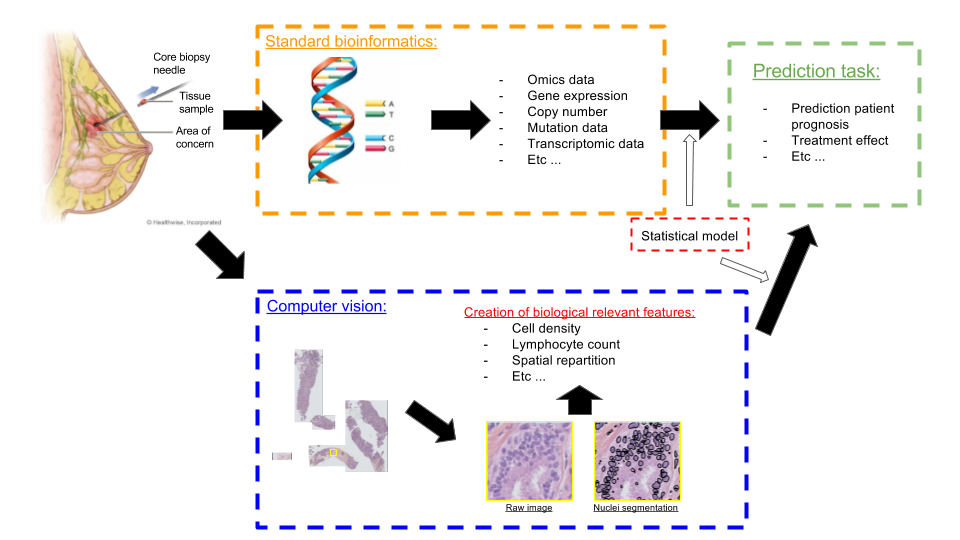
\includegraphics[width=0.9\textwidth]{Whatido.png}
\caption{Workflow}
\label{workflow1}
\end{figure*}


\begin{figure*}[!ht]
\centering
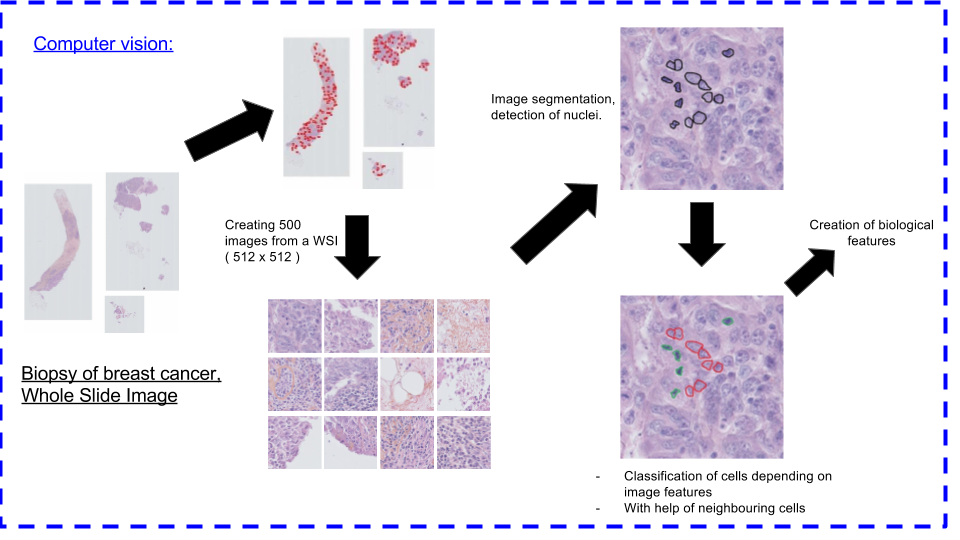
\includegraphics[width=0.8\textwidth]{ComputerVision.png}
\caption{Computer Vision aspect}
\label{fig:ComputerVision}
\end{figure*}

\begin{figure*}
    \centering
\begin{subfigure}[t]{0.45\textwidth}
        \centering
        \hspace{0.5cm}
        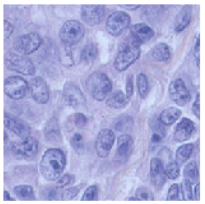
\includegraphics[width=0.6\linewidth]{RAW} 
        \caption{Raw image} \label{fig:raw}
    \end{subfigure}%
    \begin{subfigure}[t]{0.45\textwidth}
        \centering
        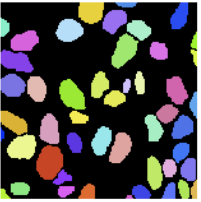
\includegraphics[width=0.6\linewidth]{LBL} 
        \caption{Ground Truth} \label{fig:lbl}
    \end{subfigure}

%    \vspace{1cm}
    \begin{subfigure}[t]{\textwidth}
    \centering
       \hspace{-0.6cm}
       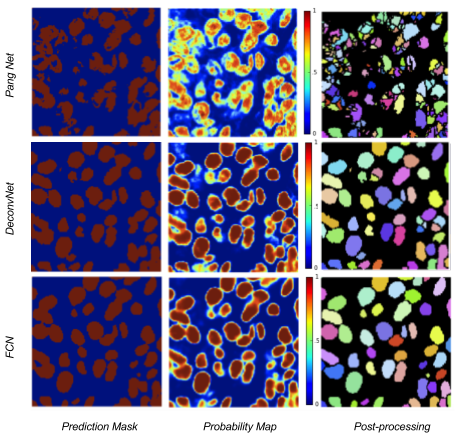
\includegraphics[width=0.8\linewidth]{Test} 
        \caption{Some outputs} \label{fig:outputs}
    \end{subfigure}
    \caption{Nuclei segmentation}
    \label{fig:all}
\end{figure*}


 \begin{table*}[!ht]
\centering
\begin{tabular}{|c|c|c|c|c|c|}
\hline
  & PangNet & U-Net & DeconvNet & FCN & Ensemble\\
 \hline
Accuracy  &  0.924 & 0.919 & 0.954 &0.944 & 0.944  \\
IU   &    0.722 & 0.568 & 0.814 & 0.782 & 0.804 \\
Recall     &  0.655 & 0.240 & 0.773 & 0.752 & 0.900 \\
Precision   &  0.814 & 0.721 & 0.864 & 0.823 & 0.741 \\
F1    &  0.676 & 0.360 & 0.805 & 0.763  & 0.802\\
% TP       &       0.744 &     0.856 & 0.855 & 0.876 \\
% TN      &       0.963 &     0.981 &  0.977 & 0.979\\
Performance    &  0.803 & 0.615 & 0.875 & 0.862 & 0.922 \\
% Pixel error  &  0.063 &     0.032 & 0.042 & 0.032\\
\hline
\end{tabular}
\caption{Results}
\label{tab:res}
\end{table*}



\clearpage



\section*{List of publications}

\begin{itemize}
\item Peter Naylor, Marick Laé, Fabien Reyal and Thomas Walter. Nuclei Segmentation in Histopathology Images using Deep Neural Networks. In \textit{International Symposium on Biomedical Imaging (ISBI'17), Melbourne, Australia}, April 18-21, 2017.
\end{itemize}
\end{document}